% mnras_template.tex
%
% LaTeX template for creating an MNRAS paper
%
% v3.0 released 14 May 2015
% (version numbers match those of mnras.cls)
%
% Copyright (C) Royal Astronomical Society 2015
% Authors:
% Keith T. Smith (Royal Astronomical Society)

% Change log
%
% v3.0 May 2015
%    Renamed to match the new package name
%    Version number matches mnras.cls
%    A few minor tweaks to wording
% v1.0 September 2013
%    Beta testing only - never publicly released
%    First version: a simple (ish) template for creating an MNRAS paper

%%%%%%%%%%%%%%%%%%%%%%%%%%%%%%%%%%%%%%%%%%%%%%%%%%
% Basic setup. Most papers should leave these options alone.
\documentclass[a4paper,fleqn,usenatbib]{mnras}

% MNRAS is set in Times font. If you don't have this installed (most LaTeX
% installations will be fine) or prefer the old Computer Modern fonts, comment
% out the following line
%\usepackage{newtxtext,newtxmath}
% Depending on your LaTeX fonts installation, you might get better results with one of these:
%\usepackage{mathptmx}
\usepackage{txfonts}

% Use vector fonts, so it zooms properly in on-screen viewing software
% Don't change these lines unless you know what you are doing
\usepackage[T1]{fontenc}
\usepackage{ae,aecompl}
%\usepackage{subfig,multirow}
\usepackage{pdflscape}


%%%%% AUTHORS - PLACE YOUR OWN PACKAGES HERE %%%%%

% Only include extra packages if you really need them. Common packages are:
\usepackage{graphicx}	% Including figure files
%\usepackage{wasysym}
\usepackage{savesym}
\savesymbol{iint}
\savesymbol{iiint}
\savesymbol{iiiint}
\savesymbol{idotsint}
\usepackage{amsmath}	% Advanced maths commands
\usepackage{amssymb}	% Extra maths symbols
\usepackage{amsmath,color}
\usepackage{graphicx}
%\usepackage[showframe]{geometry}% http://ctan.org/pkg/geometry
\usepackage{lipsum}% http://ctan.org/pkg/lipsum
\usepackage{graphicx}% http://ctan.org/pkg/graphicx
%\usepackage[demo]{graphicx}
%\usepackage{subfigure}
\usepackage{marvosym}
\usepackage{mathtools}
\usepackage{cancel}
\usepackage{bm}
\usepackage[T1]{fontenc}
\usepackage{aecompl} 
\usepackage{arydshln}
\usepackage{subfig,multirow}
\usepackage{mathrsfs}
\usepackage{algorithm}
\usepackage[noend]{algpseudocode}


%%%%%%%%%%%%%%%%%%%%%%%%%%%%%%%%%%%%%%%%%%%%%%%%%%

%%%%% AUTHORS - PLACE YOUR OWN COMMANDS HERE %%%%%

% Please keep new commands to a minimum, and use \newcommand not \def to avoid
% overwriting existing commands. Example:
%\newcommand{\pcm}{\,cm$^{-2}$}	% per cm-squared
\newcommand{\bz}{\bmath{z}}
\newcommand{\br}{\bmath{r}}
\newcommand{\bg}{\bmath{g}}
\newcommand{\bd}{\bmath{d}}
\newcommand{\bv}{\bmath{v}}
\newcommand{\bn}{\bmath{n}}
\newcommand{\by}{\bmath{y}}
\newcommand{\bJ}{\bmath{J}}
\newcommand{\bD}{\bmath{D}}
\newcommand{\conj}[1]{\overline{#1}}
%%%%%%%%%%%%%%%%%%%%%%%%%%%%%%%%%%%%%%%%%%%%%%%%%%

%%%%%%%%%%%%%%%%%%% TITLE PAGE %%%%%%%%%%%%%%%%%%%

% Title of the paper, and the short title which is used in the headers.
% Keep the title short and informative.
\title[Sparse Redundant Calibration]{SpARC: Sparse Redundant Calibration}

% The list of authors, and the short list which is used in the headers.
% If you need two or more lines of authors, add an extra line using \newauthor
\author[K. T. Smith et al.]{
Keith T. Smith,$^{1}$\thanks{E-mail: mn@ras.org.uk (KTS)}
A. N. Other,$^{2}$
Third Author$^{2,3}$
and Fourth Author$^{3}$
\\
% List of institutions
$^{1}$Royal Astronomical Society, Burlington House, Piccadilly, London W1J 0BQ, UK\\
$^{2}$Department, Institution, Street Address, City Postal Code, Country\\
$^{3}$Another Department, Different Institution, Street Address, City Postal Code, Country
}

% These dates will be filled out by the publisher
\date{Accepted XXX. Received YYY; in original form ZZZ}

% Enter the current year, for the copyright statements etc.
\pubyear{2015}

% Don't change these lines
\begin{document}
\label{firstpage}
\pagerange{\pageref{firstpage}--\pageref{lastpage}}
\maketitle

% Abstract of the paper
\begin{abstract}
This is a simple template for authors to write new MNRAS papers.
The abstract should briefly describe the aims, methods, and main results of the paper.
It should be a single paragraph not more than 250 words (200 words for Letters).
No references should appear in the abstract.
\end{abstract}

% Select between one and six entries from the list of approved keywords.
% Don't make up new ones.
\begin{keywords}
keyword1 -- keyword2 -- keyword3
\end{keywords}

%%%%%%%%%%%%%%%%%%%%%%%%%%%%%%%%%%%%%%%%%%%%%%%%%%

%%%%%%%%%%%%%%%%% BODY OF PAPER %%%%%%%%%%%%%%%%%%

\section{Introduction}

Main contributions of the paper:

\begin{enumerate}
 \item Present a general framework which unifies all the techniques developed so far showing they are all related (LINCAL, non-linear estimator, etc ...). They are all non-linear
 least-squares techniques, i.e. they either employ Gauss-Newton or the Levenberg-Marquardt algorithms. We have to start with LINCAL showing that it is GN, then we have to motivate 
 why we want to use Oleg's complex optimization framework.
 \item Use Oleg's complex optimization framework to re-derive the non-linear technique proposed by Marthi and Chengular. The novelty lies, in the fact that by using Oleg's
 framework we can find analytic expressions for the Jacobian, the Hessian and the Jacobian-residual product (which is not even the case for LINCAL). State that the algorithm is 
 effectively related to SteFCal and is eff an independent rediscovery of SteFCal and an extension of it into the redundant domain.
 \item Also we present the array geometry function to help us make the derivations from Marthi and Chengular easier to read and understand for a general layout.
 \item We also mention at this point that in Oleg's paper the question is raised is there a fast way of computing the exact inverse, we then present this new method, which is called
 conjugate gradient method. We discuss the algorithm and the two things which bound its execution time. Which is $kappa$ and $m$ (spectral condition number and its sparsity). Then
 we explore both of these parameters.
  \end{enumerate} 
 **************
 FLOW OF PAPER
 **************
 
 \begin{enumerate}
 \item We need the definition of visibilities as in Liu. DEFINE SNR HERE ALREADY together maybe with the sigma value of the noise.
 \item Introduce the array geometery function.
 \item Write down logcal and lincal in matrix form... ?
 \item Short discussion of least squares and jacobian and hessian's. General GN and LM update rules.
 \item Introduce redundant calibration as a least squares problem. We will use this general fact to derive both popular methods.
 \item Propose a possible solution witch leads to lincal. Mention that this approach works as in this form the function is differentiable (a taylor expansion in the 
 parameters exists). Maybe mention that we can also divide the problem into real and imaginary etc...
 \item Show how this relates to lincal for example ---> show lincal is GN.
 \item Now introduce complex optimization ---> Main motivation for switching to the alternative framework is that the the differentials are very simplistic. We wish to show that
 we can derive the method of Chengular.
 \item Do the derivation of Chengular. 
 \item Brief discussion abouth Chengular and SteFCal and Complex Optimization. Here I show that in Oleg's paper he re-derives an algorithm called SteFCal. Stefcal works
 on the basis of alternating direction implicit method. The first signs of achieving a similar algorithm already appeared in Stefan's conference paper in which the alternating
 idea was first proposed. Then I mention Chegular re-derives the expression by using partial derivatives and extends it to redundant. One could also have used the linear alternating
 approach. In an attempt to merge the terminology that has independently develop in the general calibration and redundant calibration literature and to emphasize the close
 relationship between Stefcal and the approach derived by I will use the label Redunandat SteFCal (R-Stefcal) to refer to the NLS method proposed by ... Lastly we mention that similarly
 to how Oleg re-derived stefcal in, we have achieved the same approach.
 \item Faster Exact inverse. A question that Oleg poses in his paper is, does there exist a faster way to take the exact inverse of JhJ? One that is almost linear, and
 implies that we can therefore implement the full LM algorithm. The aim here is of course to reduce the number of iterations that are required to converge by using the 
 full inverse instead which would hopefully provide enough of a speedup to compensate for the more expensive full-inverse. The algorithm we propose is the conjugate 
 gradient method.
 \item We give the images of the HESSIAN of both lincal and the complex method (number of terms). So we can mention that both are sparse and contain diagonal entries that 
 are more significant than the off-diagonal entries. What linear inversion approach can take advantage of both these phenomenon. One such technique is 
 cg. 
 \item Briefly discuss CG and how its computationally bounded by its condition number and its sparsity (how does the diagonal play a role).
 \item Simulation description
 \item Will CG improve things?
 \item Now first discuss the condition
 number of the Hessian before and after pre-conditioning (pre-codnitioning can only be applied if a good inverse of a matrix is known, if it is known then it can improve 
 the spectral condition number of a matrix. We present here the kappa and iteration number graphs for the HEXAGONAL layout. Although the
 \item Now we discuss the sparsity results. 
 \item Provide a table that theoretical compares R-StEFCal and SPARC.
 \item Number of outerloop iterations. 
 \item Timing results.
 \item Accuracy results.
 \item Maybe some freq simulations.
 \end{enumerate}
 
 We
 
 We neeed LOGCAL and LINCAL in matrix forms
 
 
 


%All papers should start with an Introduction section, which sets the work
%in context, cites relevant earlier studies in the field by \citet{Others2013},
%and describes the problem the authors aim to solve \citep[e.g.][]{Author2012}.

\section{Visibilities}
The observed visibility $d_{pq}$ measured by the baseline formed by antenna $p$ and $q$ can be described as

\begin{equation}
\label{eq:vis_definition}
d_{pq} = g_{p}\conj{g}_{q}y_{pq} + n_{pq},
\end{equation}
where $g_{p}$ and $g_{q}$ are the direction independent gains associated with antenna $p$ and $q$, $y_{pq}$ denotes the true visibility that baseline $pq$ measured
and $n_{pq}$ is the thermal noise component. Conjugation is denoted by $\conj{(*)}$. During the course of an actual observation the true value of $g_p$, $g_q$ and $y_{pq}$ are unknown and are the quantities which infact have 
to be estimated.

The real and imaginary components of the thermal noise is normally distributed with a mean of zero and a standard deviation that is equal to [NB - are the real and imaginary parts defined with same sigma?]  
\begin{equation}
\sigma = \frac{\sqrt{2}k_{B}T_{\textrm{sys}}}{A\eta\sqrt{\Delta \nu \tau}}, 
\end{equation}
where $k_B$ is Boltzmann's constant, $T_{\textrm{sys}}$ is equal to the system temperature, $A$ is the effective collecting area of each element in the array, $\eta$ is a dimensionless
efficiency factor, $\Delta \nu$ is the observational bandwidth and $\tau$ is the integration time per visibility. 

\subsection{Redundant Array Geometry Mapping}
If an array is redundant then its redundant baselines sample the exact same visibilites in the $uv$-plane, i.e. if baseline $pq$ and $rs$ are redundant then $y_{pq} = y_{rs}$. We can
therefore also use the following useful indexing strategy: We can use singular redundant baseline indexes instead of composite antenna pairs to label the true observed visibilities. 

Let $\phi_{ij}:\mathbb{N}^2\rightarrow\mathbb{N}^+$ be the mapping that maps composite antenna pairs to the unique redundant baseline indexes of an array. This mapping is not symmetric as 
$\phi_{ij} = 0$ if $i>j$. It is possible to construct a simple analytic expression for $\phi_{ij}$ when our array is in an east-west regular configuration:
\begin{equation}
\phi_{ij} = 
\begin{cases}
j-i&\textrm{if}~i<j\\
0&\textrm{otherwise}
\end{cases}.
\end{equation}
It becomes increasingly more difficult to construct analytic expressions of $\phi_{ij}$ for other more complicated array layouts.

We can also define the following symmetric variant of $\phi_{ij}$:
\begin{equation}
\zeta_{ij} = 
\begin{cases}
\phi_{ij}~\textrm{if}~i\leq j\\
\phi_{ji}~\textrm{if}~i>j
\end{cases}.
\end{equation} 

%\begin{figure*}
%\centering
%\subfig[full-complex:   Real]
%{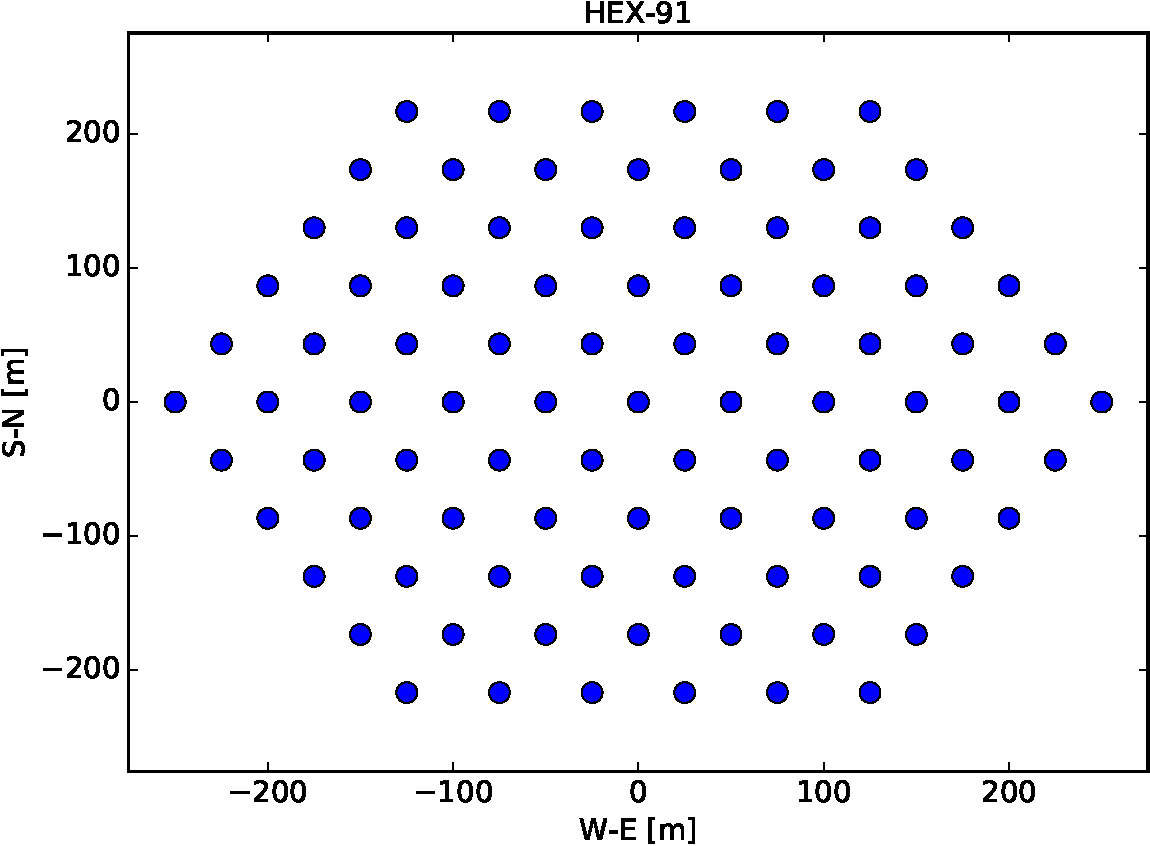
\includegraphics[width=0.34\textwidth]{./HEX_lay.pdf}\label{fig:stef_r}}
% V_R_3.pdf: 585x441 pixel, 72dpi, 20.64x15.56 cm, bb=0 0 585 441
%\subfig[full-complex:  Imag]
%{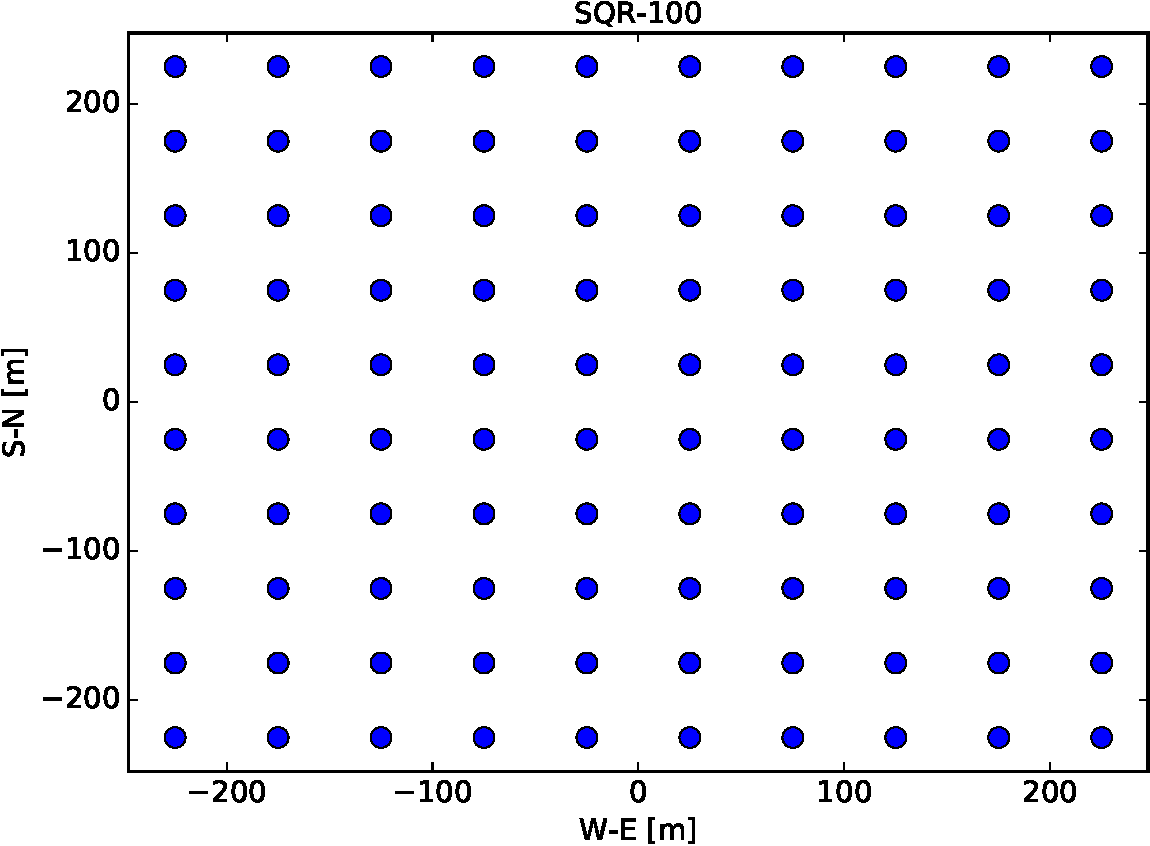
\includegraphics[width=0.34\textwidth]{./SQR_lay.pdf}\label{fig:stef_i}}
% V_R_3.pdf: 585x441 pixel, 72dpi, 20.64x15.56 cm, bb=0 0 585 441
%\subfig[full-complex: ghost pattern]
%{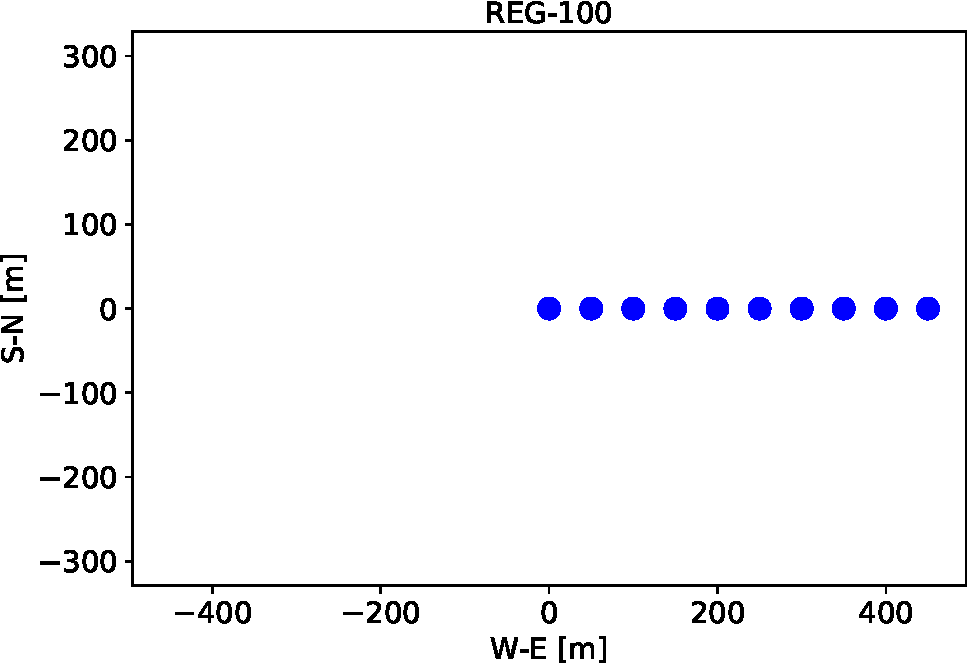
\includegraphics[width=0.34\textwidth]{./REG_lay.pdf}\label{fig:full_pat_45}}\\
% V_R_3.pdf: 585x441 pixel, 72dpi, 20.64x15.56 cm, bb=0 0 585 441
%\subfig[phase-only:   Real]
%{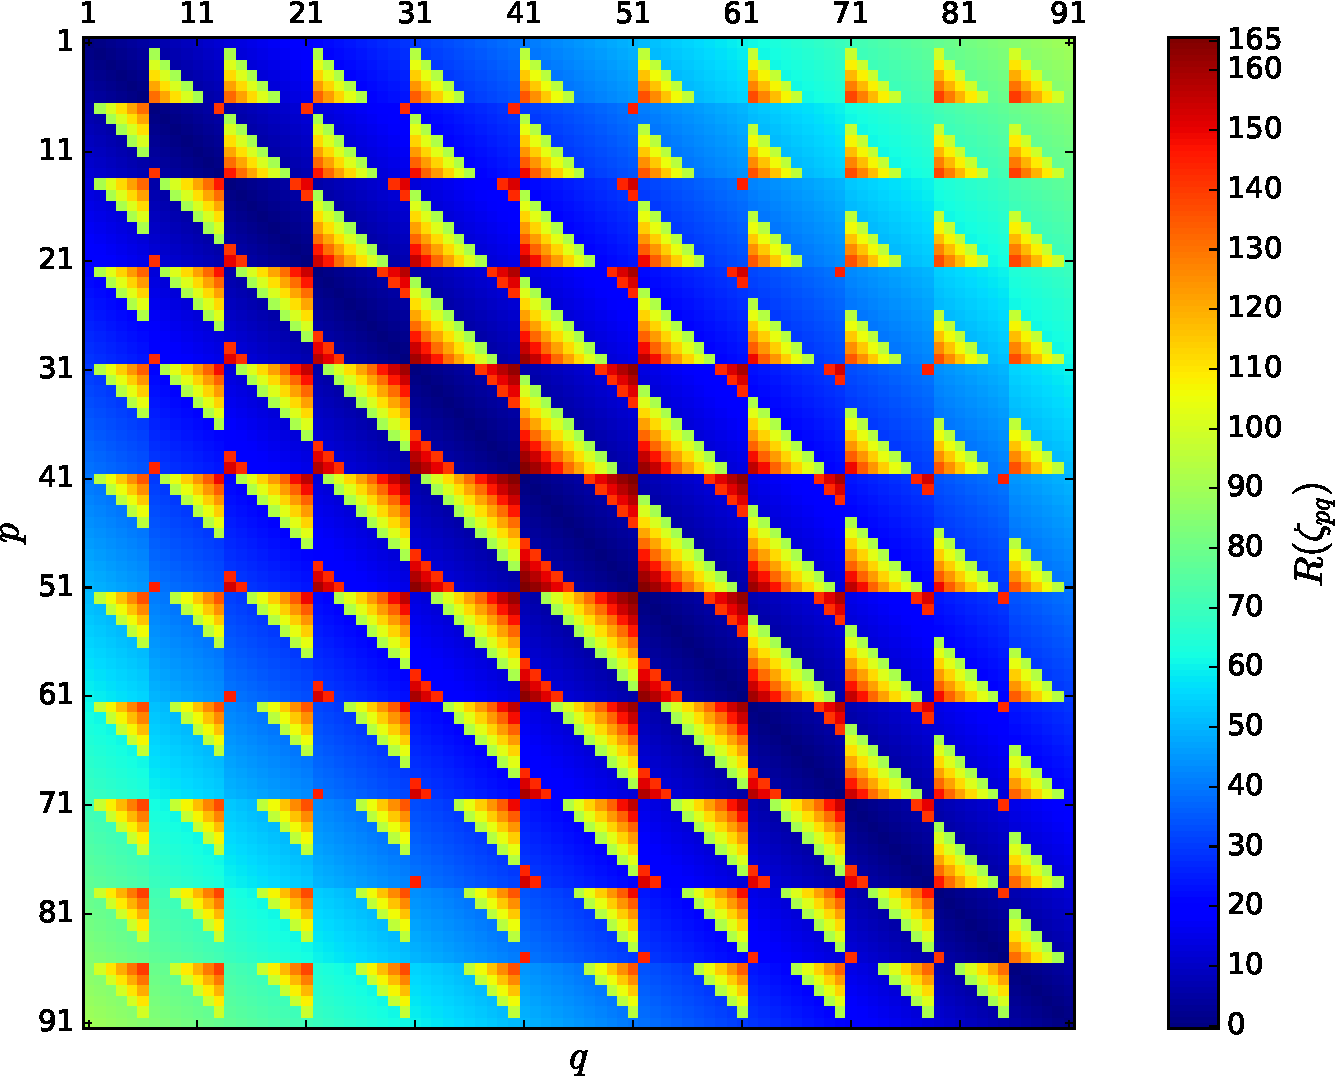
\includegraphics[width=0.34\textwidth]{./HEX_phi.pdf}\label{fig:phase_r}}
% V_R_3.pdf: 585x441 pixel, 72dpi, 20.64x15.56 cm, bb=0 0 585 441
%\subfig[phase-only:   Imag]
%{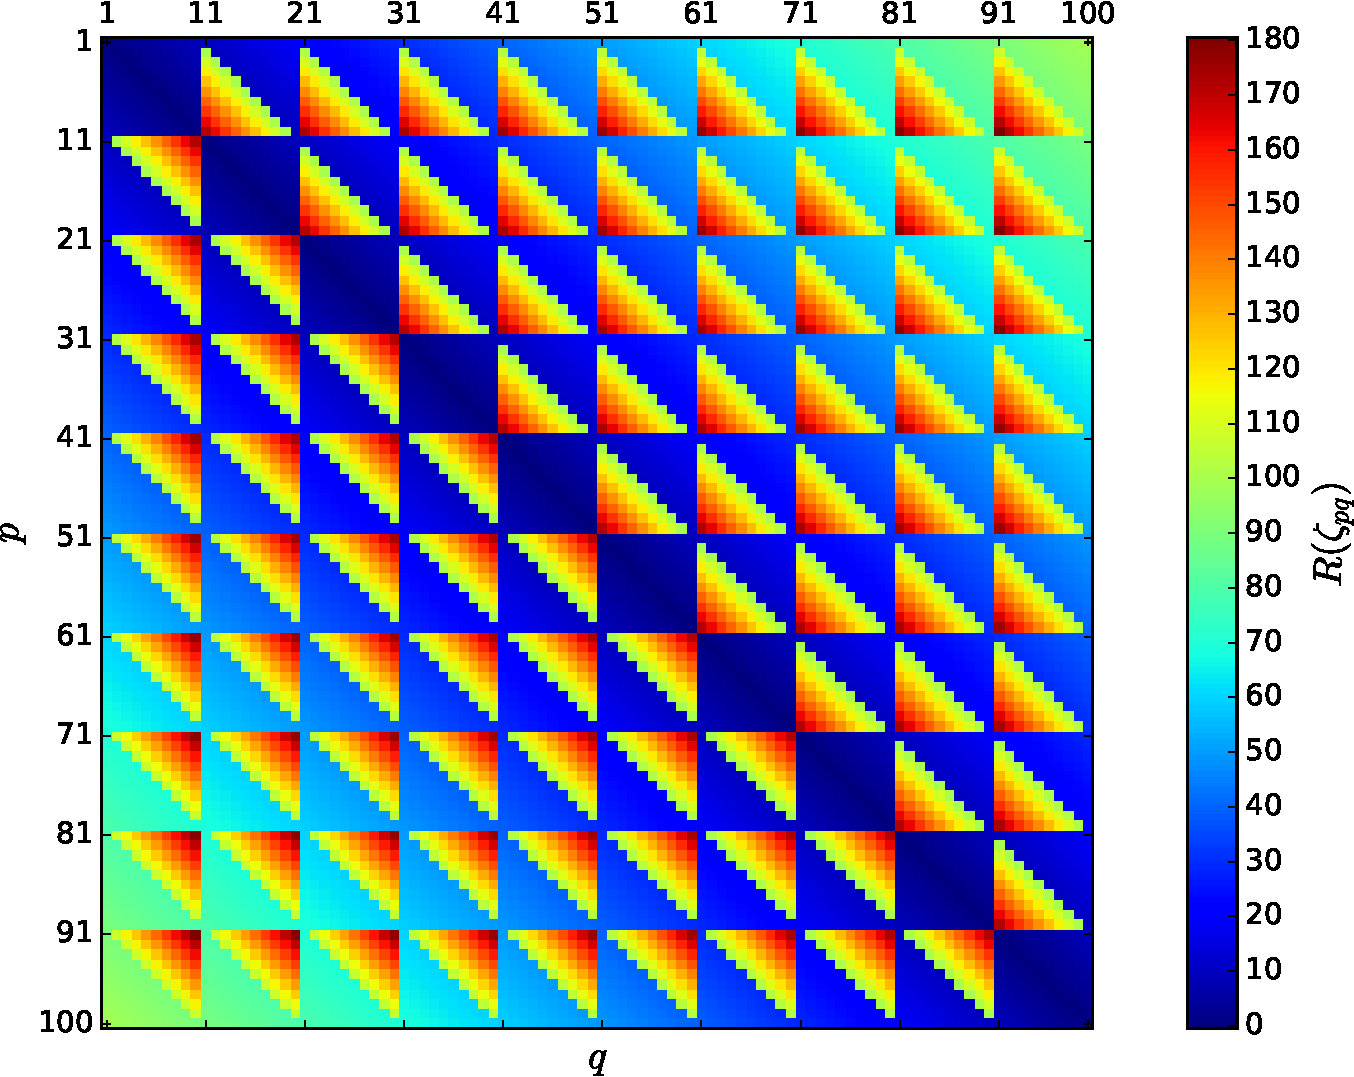
\includegraphics[width=0.34\textwidth]{./SQR_phi.pdf}\label{fig:phase_i}}
% V_R_3.pdf: 585x441 pixel, 72dpi, 20.64x15.56 cm, bb=0 0 585 441
%\subfig[phase-only: ghost pattern]
%{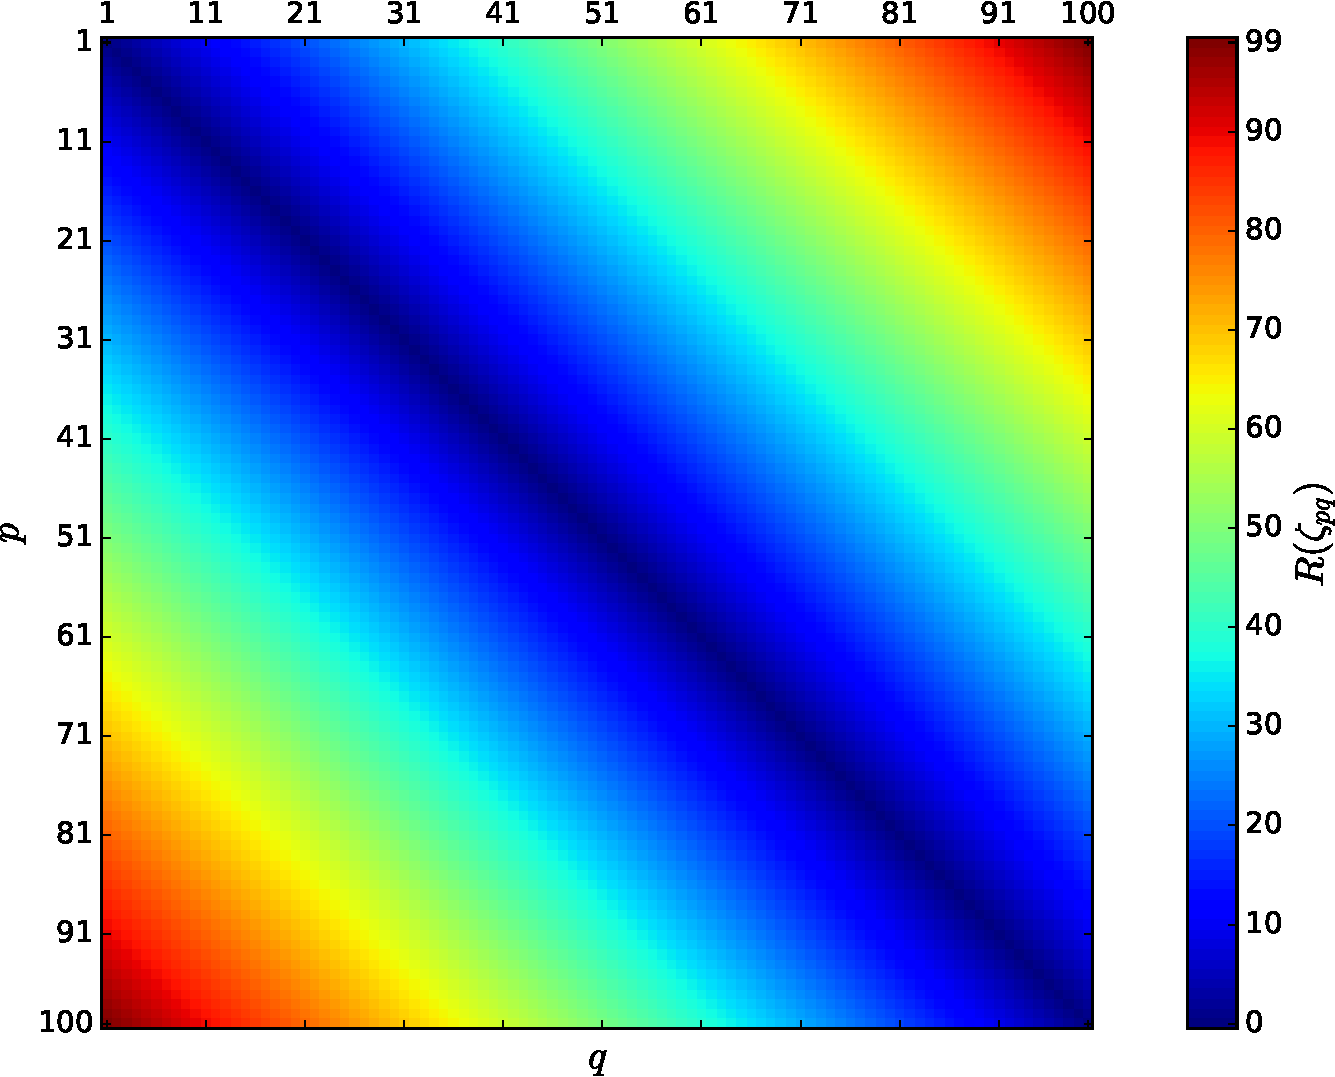
\includegraphics[width=0.34\textwidth]{./REG_phi.pdf}\label{fig:phase_pat_45}}
% V_R_3.pdf: 585x441 pixel, 72dpi, 20.64x15.56 cm, bb=0 0 585 441
%\caption{scenario. \label{fig:ghost_pattern_bas_45}}
%\end{figure*}

\begin{figure*}%
\centering
\subfloat[./HEX_lay.pdf]{}%
\qquad
\subfloat[./SQR_lay.pdf]{}
\caption{Here are the first two figures of a continued figure.}%
\label{fig:cont}%
\end{figure*}

If the mapping $\phi_{ij}$ is known and one is given one of the two antenna indexes that together form a redundant baseline as well as the redundant baseline index itself then it is possible 
to calculate the unknown antenna index. This can be calculated via the following two expressions:
\begin{equation}
\xi_{ij} = 
\begin{cases}
p~\textrm{if}~\exists! ~ p \in \mathbb{N} ~ s.t. ~(\phi_{pi} = j)\\
0~\textrm{otherwise}
\end{cases},
\end{equation}
and
\begin{equation}
\psi_{ij} = 
\begin{cases}
q~\textrm{if}~\exists! ~ q \in \mathbb{N} ~ s.t. ~(\phi_{iq} = j)\\
0~\textrm{otherwise}
\end{cases}
\end{equation}

We use $\xi_{ij}$ to retrieve the first antenna index of the composite antenna pair associated with a particular baseline if the index of the first antenna in the composite antenna pair and the unique redundant baseline index are known, while we use $\psi_{ij}$ to obtain 
a similar result; the second antenna index of the composite antenna pair. \textbf{NB::} I still need to plot $\zeta_{ij}$ for different antenna layouts.

If the array is redundant and the mapping $\phi_{ij}$ is known we can rewrite Eq.~\eqref{eq:vis_definition} as
\begin{equation}
\label{eq:vis_red}
d_{pq} = g_{p}\conj{g}_{q}y_{\phi_{pq}} + n_{pq}.
\end{equation}
Eq.~\eqref{eq:vis_red} can also be expressed in the following vector form 
\begin{equation}
\bd = \bv + \bn, 
\end{equation}
where 
\begin{eqnarray}
 \bd &=& [d_{pq}] \big \} ~ [pq] = 1\cdots B ~ (p<q),\nonumber\\
 \bv &=& [g_p y_{\phi_{pq}} \conj{g}_q]  \big \} ~ [pq] = 1\cdots B ~ (p<q),\nonumber\\
 \bn &=& [n_{pq}]  \big \} ~ [pq] = 1\cdots B ~ (p<q).\label{eq:vec_definitions}
\end{eqnarray}
In Eq.~\eqref{eq:vec_definitions}, $B$ denotes the number of baselines in the array.

We will be using the following SNR (signal-to-noise ratio) definition in this paper  
\begin{equation}
\textrm{SNR} = \frac{<\bv\odot\conj{\bv}>_{t,pq}}{<\bn\odot\conj{\bn}>_{t,pq}}, 
\end{equation}
where $<*>_{t,pq}$ denotes averaging over time and baselines and $\odot$ denotes the Hadamard product. The definition we use here is similar 
to the SNR definitions of \citet{Liu2010,Marthi2014}.




\section{Historical Overview}

Write a little about how redundant calibration developed, a basic lit review.
Maybe write a little bit about LOGCAL here as well.

\subsection{EW regular-layout}
Describe the EW-layout and its redundant baselines

\subsection{LINCAL}
\begin{equation}
c_{ij} = y_{i-j} e^{\eta_i - i \varphi_i} e^{\eta_j - i \varphi_j}
\end{equation}

\begin{eqnarray}
\frac{c_{ij}}{\partial \eta_i} &=& y_{i-j} e^{\eta_i - i \varphi_i} e^{\eta_j - i \varphi_j}\\ 
\frac{c_{ij}}{\partial \varphi_i} &=&  -i y_{i-j} e^{\eta_i - i \varphi_i} e^{\eta_j - i \varphi_j}\\
\frac{c_{ij}}{\partial \eta_j} &=& y_{i-j} e^{\eta_i - i \varphi_i} e^{\eta_j - i \varphi_j}\\ 
\frac{c_{ij}}{\partial \varphi_j} &=&  i y_{i-j} e^{\eta_i - i \varphi_i} e^{\eta_j - i \varphi_j}\\
\frac{y_{i-j}}{\partial \varphi_j} &=&  e^{\eta_i - i \varphi_i} e^{\eta_j - i \varphi_j}
\end{eqnarray}

The Wirtinger derivative is used in the last equation.

\begin{eqnarray}
c_{ij} &\approx& c_{ij}^0 + \Delta \eta_i(y_{i-j}^0 e^{\eta_i^0 - i \varphi_i^0} e^{\eta_j^0 - i \varphi_j^0}) + \Delta \eta_j(y_{i-j}^0 e^{\eta_i^0 - i \varphi_i^0} e^{\eta_j^0 - i \varphi_j^0})\\
&& -i\Delta\varphi_i (y_{i-j}^0e^{\eta_i^0 - i \varphi_i^0} e^{\eta_j^0 - i \varphi_j^0}) +i\Delta\varphi_j (y_{i-j}^0e^{\eta_i^0 - i \varphi_i^0} e^{\eta_j^0 - i \varphi_j^0})\\
&& y_{i-j}^1(y_{i-j}^0e^{\eta_i^0 - i \varphi_i^0} e^{\eta_j^0 - i \varphi_j^0})\\
&\approx&  c_{ij}^0 + e^{\eta_i^0 - i \varphi_i^0} e^{\eta_j^0 - i \varphi_j^0}(y_{i-j}^1 + y_{i-j}^0( \Delta \eta_i+ \Delta \eta_j - i\Delta\varphi_i + i\Delta\varphi_i))
\end{eqnarray}

\begin{equation}
\label{eq:residual}
r_{ij} = \delta_{ij} = c_{ij}-c_{ij}^0 = e^{\eta_i^0 - i \varphi_i^0} e^{\eta_j^0 - i \varphi_j^0}(y_{i-j}^1 + y_{i-j}^0( \Delta \eta_i+ \Delta \eta_j - i\Delta\varphi_i + i\Delta\varphi_i)) 
\end{equation}

Eq.~\ref{eq:residual} allows us to construct the following linear system:

\begin{equation}
\boldsymbol{J}[\boldsymbol{\Delta \eta},\boldsymbol{\Delta \varphi},\boldsymbol{\Delta y}]^T = \boldsymbol{r}, 
\end{equation}

where $\boldsymbol{J}$ is equal to 
\begin{equation}
\boldsymbol{J} = \bigg [\overbrace{\frac{c_{pq}}{\partial \eta_i}}^{i= 1\cdots N},~\overbrace{\frac{c_{pq}}{\partial \varphi_i}}^{i= 1\cdots N},~\overbrace{\frac{c_{pq}}{\partial y_{t}}}^{t=1\cdots r_s} \bigg ] \bigg \} [pq] = 1\cdots N_{\textrm{b}} (p<q) 
\end{equation}
or
\begin{equation}
\boldsymbol{J} = \bigg [\frac{c_{pq}}{\partial \boldsymbol{\eta}},~\frac{c_{pq}}{\partial \boldsymbol{\varphi}},~\frac{c_{pq}}{\partial \boldsymbol{y}} \bigg ] \bigg \} [pq] = 1\cdots N_{\textrm{b}} (p<q). 
\end{equation}

The last column is again a Wirtinger derivative.

Which means we can obtain the least-squares estimate as follows:

\begin{equation}
[\boldsymbol{\Delta \eta},\boldsymbol{\Delta \varphi},\boldsymbol{\Delta y}]^T = [\boldsymbol{J}^H\boldsymbol{J}]^{-1}\boldsymbol{J}^H\boldsymbol{r}.
\end{equation}

What is interesting about LINCAL is that it seems to be a combination of standard least-squares (splitting the problem into amplitude and phase) and 
complex least-squares. The gains are solved with a standard approach (splitting into amp and phase) and the redundant visibilities use a Wirtinger derivative. What is strange though is that in normal complex optimization, if we optimize towards a complex variable x we also need to optimize towards
its complex conjugate. My best guess is that LINCAL works in any case since the conjugate redundant baselines are not used to calibrate ($p<q$). The only difference between the framework I was using is that
we regard the whole problem as complex, we construct our Jacobian by calculating the derivative towards $g$ and its conjugate as well as $y$ and its conjugate - Smirnov \& Tasse (2016). 

Now that the relation between LINCAL and GN has been shown we can start focusing on the speedup that the conjugate gradient method provides as Liu (2010) originally proposed.
Also worth checking: whether using an LM step instead of a GN step improves your convergence properties.
Briefly review LINCAL here and show that it is equivalent to the GN algorithm.

\section{Complex Optimization}
\subsection{Scalar Calibration}
Scalar direction independent calibration is achieved through solving the following minimization problem:
\begin{equation}
\min_{\bg}\|\br\| = \min_{\bg}\|\bd - \bv(\bg)\|, 
\end{equation}
where
\begin{enumerate}
 \item $\bd$ is the observed visibility vector, i.e. 
 \begin{equation}
  \bd = [d_{pq}] \big \} ~ [pq] = 1\cdots N ~ (p<q).
 \end{equation}
 The vector entry $d_{pq}$ denotes the observed visibility associated with the baseline formed by antenna $p$ and $q$, while $N$ denotes the number or antennas
 in the array. 
 \item $\bg = [g_1,g_2,\cdots,g_N]$ represents the instrumental complex antenna gain vector.
 \item $\bv(\bg)$ denotes the predicted visibility vector, i.e.
 \begin{equation}
  \bv(\bg) = [g_p y_{pq}\conj{g}_q]  \big \} ~ [pq] = 1\cdots N ~ (p<q).
 \end{equation}
 In Eq... $y_{pq}$ denotes the visibility which was created from a skymodel and is associated with antenna $p$ and $q$. [Need to rw this sentence] 
\end{enumerate}

One of the simplests approaches one could use to solve eq. is to use least-squares optimization which we can only employ if we are able to calculate the gradient of $\bv(\bg)$,
implying that $\bv(\bg)$ needs to be analytic in $\bg$ (the Taylor series expansion of $\bv(\bg)$ exists).
The problem we face if we try to naivly apply least-squares to eq is that $\bv(\bg)$ is not analytic in its argument, since $\frac{\partial \conj{z}}{\partial z}$ (where 
$z \in \mathbb{C}$) does not exist.

The easiest way to circumvent this problem is to recast our problem in such a way that the predicted visibility vector becomes analytic in its argument.
The most widely used way to accomplish this is to restate eq as
\begin{equation}
\min_{\hat{\bg}}\|\hat{\br}\| = \min_{\hat{\bg}}\|\hat{\bd} - \hat{\bv}(\hat{\bg})\|, 
\end{equation}
where $\hat{\bg} = \big[\mathcal{R}\{\bg\},\mathcal{I}\{\bg\}\big]^T$, still need to define the other vectors properly....
Note that $\hat{\bv}(\hat{\bg})$ is now analytic in its argument and we can proceed and use least squares to estimate $\bg$. 

\citet{Smirnov2015} have recently shown that calibration can also be performed using the following complex framework: 
\begin{equation}
\min_{\breve{\bg}}\|\breve{\br}\| = \min_{\breve{\bg}}\|\breve{\bd} - \breve{\bv}(\breve{\bg})\|, 
\end{equation}
where $\breve{\bg} = \big[\bg,\conj{\bg}]^T$, still need to define the other vectors properly....
In the above formulation v breve is analytic in its argument and its complex conjugate as a whole under the assumption that the Wirtinger derivative
is used to define the gradient operator. As v breve is analytic we will are also able to apply the least squares method to .   

The Wirtinger derivatives are defined as
\begin{eqnarray}
\frac{\partial}{\partial z} = \frac{1}{2}\left ( \frac{\partial}{\partial x} -  i \frac{\partial}{\partial y} \right ),&~&\frac{\partial}{\partial \conj{z}} = \frac{1}{2}\left ( \frac{\partial}{\partial x} +  i \frac{\partial}{\partial y} \right ) 
\end{eqnarray}
where $z = x + iy$ and $x,y \in \mathbb{R}$. It follows from the above that $\frac{\partial z}{\partial z} = 1,\frac{\partial z}{\partial \conj{z}} = 0,\frac{\partial \conj{z}}{\partial z} = 0$ and $\frac{\partial \conj{z}}{\partial \conj{z}} = 1$.





%The main difference between the traditional approach and the 
%complex optimization framework proposed by \citet{Smirnov2015} is that in their framework they no longer treat the real and imaginary parts of the residual separately which enables them to directly solve for the complex antenna gains themselves (as well as their
%complex conjugates). 


Recall that most optimization techniques require a gradient operator to enable it to function properly. The main reason why we have traditionally treated 
the real and imaginary parts of the residual separately is due to the fact that $f(z) = \conj{z}$ is not a differentiable complex function where $z\in\mathbb{C}$ and $\conj{(*)}$ denotes conjugation, i.e. $\frac{df(z)}{dz}$
does not exist, if we apply the standard definition of differentiation:
\begin{equation}
x
\end{equation}



The main reason that we do not need to treat the real and imaginary parts of the residual separately any more is due to the 
fact 

%A standard way to optimize a complex function $f(\bz)$ of $n$ complex variables $\bz\in\mathbb{Z}^n$ is to recast $f$ as  optimize the real and imaginary parts of  separately.

 

The main difference between complex optimization and the more traditional
approach to calibration is that in complex calibration we 

\subsection{Redundant Calibration}
In eq a sky model is required to generate the predicted visibilities $y_{pq}$ as we have too few equations to also solve for them and the gains. If we use a redundant layout
we can reduce the number of unknowns so that we are able to solve for the sky and the gains simultaneously.

\subsubsection{Antenna indices to redundancy index mapping}
If an array is redundant its redundant baselines sample the exact same visibilites in the $uv$-plane. Recall, that we denote the true observed visibility associated with baseline $pq$ and 
baseline $rs$ with $y_{pq}$ and $y_{rs}$, respectively . However if baseline $pq$ and $rs$ represent the same redundant baseline then $y_{pq} = y_{rs}$. Another
usefull indexing strategy would therefore be to use redundant baseline indices instead of antenna pairs to label the true observed visibilities so that we can identify 
which baselines observe the same visibilities barring instrumental and environmental errors.

Let $\phi_{ij}:\mathbb{N}^2\rightarrow\mathbb{N}^+$ be the mapping that maps antenna indices to the unique redundant baseline indices of the array. This mapping is not symmetric as 
$\phi_{ij} = 0$ if $i>j$. For an east-west regular array we can construct a simple analytic expression for this mapping:
\begin{equation}
\widehat{\phi_{ij}} = 
\begin{cases}
j-i&\textrm{if}~i<j\\
0&\textrm{otherwise}
\end{cases}.
\end{equation}
As will become apparent later the following symmetric variant of $\phi_{ij}$ will turn out to be quite useful later on:
\begin{equation}
\zeta_{ij} = 
\begin{cases}
\phi_{ij}~\textrm{if}~i\leq j\\
\phi_{ji}~\textrm{if}~i>j
\end{cases}.
\end{equation} 
It is also crucial to be able to determine the antenna index of the antenna which was used to construct a specific redundant baseline if one is given the other antenna index and the redundant baseline index. This can be calculated via the following two functions:
\begin{equation}
\xi_{ij} = 
\begin{cases}
p~\textrm{if}~\exists! ~ p \in \mathbb{N} ~ s.t. ~(\phi_{pi} = j)\\
0~\textrm{otherwise}
\end{cases},
\end{equation}
and
\begin{equation}
\psi_{ij} = 
\begin{cases}
q~\textrm{if}~\exists! ~ q \in \mathbb{N} ~ s.t. ~(\phi_{iq} = j)\\
0~\textrm{otherwise}
\end{cases}
\end{equation}
We use $\xi_{ij}$ to retrieve the index of the second antenna if we know the redundant baseline index and the index of the first antenna used to construct the baseline in question, while we use $\psi_{ij}$ to return the index of the first antenna if we know the 
index of the second antenna instead. \textbf{NB::} I still need to plot $\zeta_{ij}$ for different antenna layouts.

Describe complex optimization, Jacobian, Hessian etc... Benefits drawbacks compared to LINCAL... etc..

\subsubsection{Redundant calibration}
In the case of a redundant array we can not only solve for the gains $\bg$ but we can also solve for the redundant unknown visibilities $\by$. Where $\by = [y_1,\cdots,y_R]$, $y_i$ denotes 
a unique redundant visibility and $R$ is the maximum value of the mapping $\phi_{ij}$. The reason we can now also solve for $\by$ is because we have reduced the number of 
unknowns from $N+B$ to $N+R$, where $N+R$ is now less than $B$ due to the array redundancy. We can now reformulate the calibration problem for an redundant array as follow:
\begin{equation}
\min_{\bz}\|\br\| = \min_{\bz}\|\bd - \bv(\bz)\|, 
\end{equation}
where $\bz = [\bg,\by]^T$.

If we now follow the same extension strategy of \citet{Smirnov2015} we can rewrite eq to
\begin{equation}
\min_{\breve{\bz}}\|\breve{\br}\| = \min_{\bz}\|\breve{\bd} - \breve{\bv}(\breve{\bz})\|, 
\end{equation}
where $\breve{\bz} = [\bz,\conj{\bz}]^T$ still need to define the remaining variables properly.

We can now solve the above equation by using least-squares, which entails deriving the Gauss-Newton (GN) and Levenberg-Marquerdt (LM) update rules.
(NEED TO WRITE THIS MUCH BETTER)

\begin{equation}
\bJ = \frac{\partial\bv}{\partial\bz}~\bJ^* = \frac{\partial \bv}{\partial \breve{\bz}} 
\end{equation}

\begin{equation}
\bJ = \begin{bmatrix}
       \bJ & \bJ^* \\
       \conj{\bJ^*} & \conj{\bJ}  
      \end{bmatrix}
\end{equation}

\begin{equation}
 \Delta \breve{\bz} = \begin{bmatrix}\Delta \bz\\ \Delta \conj{\bz} \end{bmatrix} = (\bJ^H\bJ)^{-1}\bJ^H\breve{\br_k}
\end{equation}

\begin{equation}
 \Delta \breve{\bz} = \begin{bmatrix}\Delta \bz\\ \Delta \conj{\bz} \end{bmatrix} = (\bJ^H\bJ + \lambda \bD)^{-1}\bJ^H\breve{\br_k}
\end{equation}






\subsection{Jacobian derivation}
\subsection{Hessian derivation}
\begin{equation}
\boldsymbol{H} = 
\begin{bmatrix}
\boldsymbol{A} & \boldsymbol{B}\\
\boldsymbol{B}^* & \boldsymbol{A}^*
\end{bmatrix}
\end{equation}

With 

\begin{equation}
\boldsymbol{A} = 
\begin{bmatrix}
\boldsymbol{C} & \boldsymbol{D}\\
\boldsymbol{D^H} & \boldsymbol{E}
\end{bmatrix}
\end{equation}

\begin{equation}
\boldsymbol{B} = 
\begin{bmatrix}
\boldsymbol{F} & \boldsymbol{G}\\
\boldsymbol{G}^T & \boldsymbol{0}
\end{bmatrix}
\end{equation}

\begin{equation}
[\boldsymbol{C}]_{ij} = 
\begin{cases}
 \sum_{k \neq i} \left | g_k \right |^2 \left | y_{\zeta_{ik}} \right |^2 & \textrm{if} ~ i=j\\
 0 & \textrm{otherwise}
\end{cases}
\end{equation}

\begin{equation}
[\boldsymbol{D}]_{ij} = 
\begin{cases}
 g_i y_j^*  \left | g_{\psi_{ij}} \right |^2  & \textrm{if} ~ \psi_{ij}\neq0\\
 0 & \textrm{otherwise}
\end{cases}
\end{equation}

\begin{equation}
[\boldsymbol{E}]_{ij} = 
\begin{cases}
 \sum_{pq \in \mathcal{I}_i} \left | g_p \right |^2 \left | g_q \right |^2  & \textrm{if} ~ i=j\\
 0 & \textrm{otherwise}
\end{cases}
\end{equation}

\begin{equation}
[\boldsymbol{F}]_{ij} = 
\begin{cases}
 g_i g_j  \left | y_{\zeta_{ij}} \right |^2  & \textrm{if} ~ (i \neq j)\\
 0 & \textrm{otherwise}
\end{cases}
\end{equation}

\begin{equation}
[\boldsymbol{G}]_{ij} = 
\begin{cases}
 g_i y_j  \left | g_{\xi_{ij}} \right |^2  & \textrm{if} ~ (\xi_{ij}\neq0)\\
 0 & \textrm{otherwise}
\end{cases}
\end{equation}

Moreover, 

\begin{equation}
\mathcal{I}_i = \left\{pq\in\mathbb{N}^2|(\phi_{pq} = i) \right\}.
\end{equation}

The dimensions of the matrices:

\begin{enumerate}
\item $\boldsymbol{H}$: is a $(4N-2)\times(4N-2)$ or a $P \times P$ matrix. $N$ denotes the number of antennas and $P$ denotes the number of parameters. This matrix
contains $6N^2 - 2N - 2$ non-zero entries. It contains $16N^2 - 16N + 4$ entries. We can construct this matrix with $4N^2 -  4N$ or $\frac{1}{4} P^2 -1$ elementary operations.
\item $\boldsymbol{A}$: is a $(2N-1)\times(2N-1)$ matrix. This matrix has $N^2 + N - 1$ non-zero entries. We can construct this matrix with $2\frac{1}{2} (N^2 -  N)$ elementary operations.  
\item $\boldsymbol{B}$: is a $(2N-1)\times(2N-1)$ matrix. This matrix has $2N^2 - 2N$ non-zero entries. We can construct this matrix with $1\frac{1}{2} (N^2 -  N)$ elementary operations.
\item $\boldsymbol{C}$: is a $N\times N$ matrix. This matrix has $N$ non-zero entries. We can construct this matrix with $N^2-N$ elementary operations.
\item $\boldsymbol{D}$: is a $N \times (N-1)$ matrix. This matrix has $\frac{1}{2} (N^2 -  N)$ non-zero entries. We can construct this matrix with $\frac{1}{2} (N^2 -  N)$ elementary operations. 
\item $\boldsymbol{E}$: is a $(N-1) \times (N-1)$ matrix. This matrix has $(N-1)$ non-zero entries. We can construct this matrix with $\frac{1}{2} (N^2 -  N)$ elementary operations.  
\item $\boldsymbol{F}$: is a $N \times N$ matrix. This matrix has $N^2 - N$ non-zero entries. We can construct this matrix with $\frac{1}{2} (N^2 -  N)$ elementary operations.
\item $\boldsymbol{G}$: is a $N \times (N-1)$ matrix. This matrix has $\frac{1}{2} (N^2 -  N)$ non-zero entries. We can construct this matrix with $\frac{1}{2} (N^2 -  N)$ elementary operations.
\item $\boldsymbol{0}$: is a $(N-1) \times (N-1)$ all zero matrix. 
\end{enumerate}

We can construct $\boldsymbol{C}-\boldsymbol{G}$ in $O(N^2)$ 


The sparsity ratio of $\boldsymbol{H}$ is equal to
\begin{equation}
\gamma_N = \frac{10N^2-14N+6}{16N^2-16N+4} 
\end{equation}

The asymptotic sparsity ratio of $\boldsymbol{H}$ is equal to

\begin{equation}
\gamma = \lim_{N\rightarrow \infty}\frac{5N^2-7N+3}{8N^2-8N+2} = \frac{5}{8}
\end{equation}

Asymptotically the computational cost of the matrix-vector product between $\boldsymbol{H}$ and a vector of appropriate size is $O(P^2)$. However, the computational cost converges 
very slowly to its asymptotic value, and in general is equal to $O(P^{k_N})$, where $k_N < 2$.

\begin{eqnarray}
P^{k_N}_N &=& (1 - \gamma_N)P^2_N\\
k_N &=& \log_{P_N}(1 - \gamma_N) + 2\\
k &=& \lim_{N\rightarrow \infty} \log_{P_N}(1 - \gamma_N) + 2 = 2
\end{eqnarray}

Moreover,

\begin{eqnarray}
P^{c_N}_N &=& \frac{1}{4} P_N^2 -1\\
c_N &=& \log_{P_N}\left (\frac{1}{4} P_N^2-1 \right )\\
c &=& \lim_{N\rightarrow \infty} \log_{P_N}\left (\frac{1}{4} P_N^2-1\right ) = 2
\end{eqnarray}

NB $P_c$ IS WRONG HERE DID NOT TAKE INTO ACCOUNT THE CONJUGANTION OF $\boldsymbol{B}$ (need multiply its computational complexity by two).

\subsection{Jacobian-residual product}

\subsection{Computational complexity using CG}
\subsubsection{Sparsity}
\subsubsection{Condition number}

\begin{enumerate}
 \item Plot eigenvalue distribution for different SNR and antenna numbers and different lambda values
 \item Plot computational complexity bound plus error reduction for different setups
 \item Plot number of iterations required by CG as a function of number of antennas
 \item Plot redundant baseline visibilities to show that they are approximately equal.
\end{enumerate}

NB:: Repeat the second last plot for the positive-semi definite case (GN), showing that even if the Hessian is singular we get fast convergence.

\section{Results: Regualar square grid}
If there is time

\section{Results: Hexanol grid}
NB:: Need to test if it works for this redundant layout.


\section{Conjugate Gradient method}
brief description and lit review of the method.
computational complexity of the algorithm.
sparsity and condition number.
% \section{Methods, Observations, Simulations etc.}
% 
% Normally the next section describes the techniques the authors used.
% It is frequently split into subsections, such as Section~\ref{sec:maths} below.
% 
% \subsection{Maths}
% \label{sec:maths} % used for referring to this section from elsewhere
% 
% Simple mathematics can be inserted into the flow of the text e.g. $2\times3=6$
% or $v=220$\,km\,s$^{-1}$, but more complicated expressions should be entered
% as a numbered equation:
% 
% \begin{equation}
%     x=\frac{-b\pm\sqrt{b^2-4ac}}{2a}.
% 	\label{eq:quadratic}
% \end{equation}
% 
% Refer back to them as e.g. equation~(\ref{eq:quadratic}).
% 
% \subsection{Figures and tables}
% 
% Figures and tables should be placed at logical positions in the text. Don't
% worry about the exact layout, which will be handled by the publishers.
% 
% Figures are referred to as e.g. Fig.~\ref{fig:example_figure}, and tables as
% e.g. Table~\ref{tab:example_table}.
% 
% % Example figure
% \begin{figure}
% 	% To include a figure from a file named example.*
% 	% Allowable file formats are eps or ps if compiling using latex
% 	% or pdf, png, jpg if compiling using pdflatex
% 	\includegraphics[width=\columnwidth]{example}
%     \caption{This is an example figure. Captions appear below each figure.
% 	Give enough detail for the reader to understand what they're looking at,
% 	but leave detailed discussion to the main body of the text.}
%     \label{fig:example_figure}
% \end{figure}
% 
% % Example table
% \begin{table}
% 	\centering
% 	\caption{This is an example table. Captions appear above each table.
% 	Remember to define the quantities, symbols and units used.}
% 	\label{tab:example_table}
% 	\begin{tabular}{lccr} % four columns, alignment for each
% 		\hline
% 		A & B & C & D\\
% 		\hline
% 		1 & 2 & 3 & 4\\
% 		2 & 4 & 6 & 8\\
% 		3 & 5 & 7 & 9\\
% 		\hline
% 	\end{tabular}
% \end{table}
% 
% 
% \section{Conclusions}
% 
% The last numbered section should briefly summarise what has been done, and describe
% the final conclusions which the authors draw from their work.

\section*{Acknowledgements}

The Acknowledgements section is not numbered. Here you can thank helpful
colleagues, acknowledge funding agencies, telescopes and facilities used etc.
Try to keep it short.

%%%%%%%%%%%%%%%%%%%%%%%%%%%%%%%%%%%%%%%%%%%%%%%%%%

%%%%%%%%%%%%%%%%%%%% REFERENCES %%%%%%%%%%%%%%%%%%

% The best way to enter references is to use BibTeX:

%\bibliographystyle{mnras}
%\bibliography{example} % if your bibtex file is called example.bib

\bibliographystyle{mnras}
\bibliography{paper}
% Alternatively you could enter them by hand, like this:
% This method is tedious and prone to error if you have lots of references
%\begin{thebibliography}{99}
%\bibitem[\protect\citeauthoryear{Author}{2012}]{Author2012}
%Author A.~N., 2013, Journal of Improbable Astronomy, 1, 1
%\bibitem[\protect\citeauthoryear{Others}{2013}]{Others2013}
%Others S., 2012, Journal of Interesting Stuff, 17, 198
%\end{thebibliography}

%%%%%%%%%%%%%%%%%%%%%%%%%%%%%%%%%%%%%%%%%%%%%%%%%%

%%%%%%%%%%%%%%%%% APPENDICES %%%%%%%%%%%%%%%%%%%%%

\appendix

\section{Some extra material}

If you want to present additional material which would interrupt the flow of the main paper,
it can be placed in an Appendix which appears after the list of references.

%%%%%%%%%%%%%%%%%%%%%%%%%%%%%%%%%%%%%%%%%%%%%%%%%%


% Don't change these lines
\bsp	% typesetting comment
\label{lastpage}
\end{document}

% End of mnras_template.tex
